\documentclass[14pt,fleqn]{extarticle}
\RequirePackage{prepwell-eng}

\newcommand\fxl{ -\left(x+2 \right)}
\newcommand\fxp{ -x^2 } 
\newcommand\intg{\int_{-1}^2} 

\previewoff 

\begin{document} 
\begin{snippet}
    \correct
    
    The area $(A)$ enclosed between 
    \[ \qquad y = -x^2\text{ and } x + y + 2 = 0 \]
    is given by 
    \[ \quad A = \left\vert \intg \fxl dx +\intg x^2 \cdot dx \right\vert \] 
    
    \reason
    
    \begin{center}
  \begin{tabular}{Nl}
   \toprule
        \text{Equation} & Curve \\
   \midrule 
   x + y + 2 = 0 & Straight line with $m=-1$ \\
   & Cuts \yaxis at $y=-2$ \\
    \midrule 
    y = -x^2 & Downward opening parabola \\
    & $\qquad y \leq 0$ for all $x$ \\
    \bottomrule
  \end{tabular}
\end{center}

Hence, the curves would look like 
\begin{center}
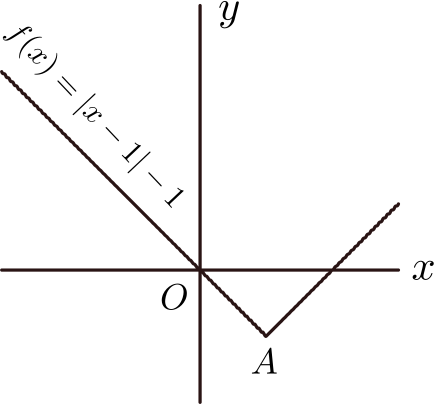
\includegraphics[scale=1.4]{figure.svg}
\end{center}

They intersect when 
\begin{align}
	y = -x^2 = \fxl &\text{ or } x^2 - x - 2 = 0  \\
	\implies (x+1)\cdot (x-2) &= 0  \\
	\text{or } x &= -1, 2 
\end{align}
    
    Which is why 
    \begin{align}
	A &= \underbrace{\left\vert \intg \fxl dx - \intg \fxp \cdot dx \right\vert}_{A\text{ is expressed as a value } > 0} \\
	&=  \left\vert \intg \fxl dx +\intg x^2 \cdot dx \right\vert
\end{align}

\end{snippet} 
\end{document} 